\chapter{Complex systems theory on adaptation and evolution (II)}

When studing complex traits (or traits, in general), it has become a reasonable assumption that there must be complex task or operation that requires such traits.
Because otherwise, such complex traits, requiring energy to maintain, would be pointless to have.
Evolutionary biologists deal with the problem of ``teleology'' in studying trait evolution \cite{Veloso2019}.
Some questions about the design of organisms and their complex traits can be raised: is there such a thing as a supernatural designer?
A similar question relating to teleology, but in a more applied aspect: is it possible to design nature the way humans, as social and intelligent beings, want?

The questions above can be answered in many different ways.
Since they will be answered in Part III of the collection, an exposition of concepts leading to the responses are presented in Part I.
Syntheses from observations in different biological and ecological systems supporting the introduction from Part I are presented in Part II.
Aside from the teleological questions, the axiom that biological and ecological systems are complex adaptive systems \cite{Dong2019} implies occurrence, given conditions, of catastrophe.
A small discussion on catastrophes will also be included in Part III.

In this chapter, connections between complex systems theory and certain biological systems are introduced.
Specifically, some aspects of complexity in biological and ecological interactions are discussed.
The conclusions from which are crucial to the development of background for later chapters.

A common trait of complex systems is non-linearity \cite{Devaney}.
In simpler contexts, nonlinear interaction between different ``agents'' of a complex system is synonymous to feedback interaction.
Such complexity can arise in different levels of organization: from chemical feedback mechanisms within an organism or cell \cite{Chaves2019}, to multicellular interaction \cite{Veloso2017}, to community interactions in different trophic levels \cite{Seibold2018}.

\section{Biological interactions}
\subsection{Biochemical pathways of metabolites}
% look up those systems that are necessary for metabolites

There is a substantial amount of literature describing the different metabolic pathways and their regulation.
Among those is a study on the mathematical modeling of feedback and feedforward interactions controlled by genes \cite{Chaves2019}.

Biochemical metabolic pathways are a series of chemical reactions catalyzed by enzymes wherein products are used for some operations inside or outside the system.
An example of a metabolic pathway is the citric acid (Krebs) cycle.
In the Krebs cycle, intermediates in the production of ATP are synthesized.
Syntheses pathways in the production of 2-Ketoglutarate, one of the important intermediates of the Krebs cycle, from xylose are studied using a newly developed algorithm \cite{Gupta2018}.
The study showed that there are different ways in producing the said intermediate.
This would mean that if such different pathways were to interfere with the citric acid cycle, feedback inhibition may occur \cite{Chaves2019}.
Conversely, the citric acid cycle may interefere with the ``different pathways''.

In the nonlinear dynamics model of \citeA{Chaves2019}, certain assumptions between interactions of intermediates of metabolite synthesis and enzymes used for metabolism were made.
In the study, metabolites in the specific metabolic system can interfere with synthesis in different parts of the pathway.
The following were taken into consideration:

\begin{itemize}
    \item Metabolites regulating enzyme activity;
    \item Enzyme kinetics;
    \item Enzyme synthesis by the cell;
    \item Metabolites regulating enzyme synthesis;
    \item Concentration dilution as an effect of cell growth
\end{itemize}

Each of the related considerations were assumed to be parameters of the system, represented as arbitrary functions or numbers.
The effects of the parameters on the sustainability of the system can be represented by graphical methods through simulations; however, figures were not present in the article being studied.
It is also very difficult to reconstruct the simulation results with the lack of control and knowledge of parameter values.
It may be sufficient to know that there exist intricate relationships between the interacting agents of the complex system, indicated by arbitrary parameters.
As a consequence from complex systems theory, different settings for parameters can lead to very varied results \cite{Devaney}. 
The extent of those effects can only be carried out through thorough analysis of the metabolism networks.   

\subsection{Developmental biology and epigenetic landscape}
From the complex system described above and the historical assumption that a gene produces one protein, and that synthesized proteins from the gene locus should be identical, why aren't identical twins completely identical?
The question posed may not have been one of the questions asked during the development of the Modern Synthesis \cite{Baedke2013, Goldberg2007}.

Identical twins have an identical genome \cite{twinz}, yet their phenotypes aren't exactly the same.
It is necessary to conclude that a single genome can give rise to multiple phenotypes.
There must be an underlying mechanism for the phenomenon.
The notion of \emph{epigenetics} was introduced some time before the Modern Synthesis \cite{Baedke2013}.
This is the mechanism in which different gene networks influence different phenotype expressions in organisms.

In embryo development, portions of DNA are attached with methyl groups to prevent their expression.
These markers are inherited from parent organisms through epigenetic inheritance \cite{Goldberg2007}.
This is one of the reasons why some offspring features look similar to their parents'.
It has also been shown that monozygotic twins share the \emph{very similar} epigenetic markers \cite{superepi}.
This is a very convincing explanation as to how identical twins appear very similar, yet not completely identical.

Going one step further by going back to the conclusion of the previous section, complexity of the system can be assumed by having different gene loci interacting with one another forming a Gene Regulatory Network (GRN) \cite{Goldberg2007}.
Similarly, gene interactions can be parametrized, simulated, and studied empirically and computationally.
The complex system can still give room to catastrophic outcomes such as one child appearing similar to grandparents from one parent and another appearing similar to grandparents from another parent.
(The example is nonsensical, but it shows an extreme possibility given certain conditions).

\section{Ecological interactions}
% look up complex systems in higher scales
% do not yet focus on the problems, but rather on how they interact
% most of the work has been summarized in Dong2019 and Seibold 2018
\subsection{Population ecology}

% the onw with spatial heterogeneity and competition Dong2019
As organisms grow and reproduce, the resources they require for further growth and respiration increases.
Suppose the case of mussels (\textit{Mytilus edulis}) a marine sessile organism \cite{Seibold2018} (Figure \ref{fig:myt}).
It would be quite illogical to clump together as a species since the resource demand of adult mussels is more than the needs of juvenile mussels.

\begin{figure}
    \centering
    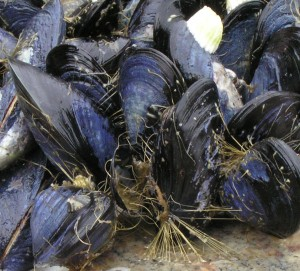
\includegraphics[scale=0.5]{mytilus}
    \caption{\textit{M. edulis} and byssal threads}
    \label{fig:myt}
\end{figure}

It would be better to disperse offspring, as in the case of seed plants.
Yet competition is only one of the mechanisms involved in population regulation.
Scale-dependent feedback regulation arises from two mechanisms: distributing resources and lessening stress.
A schematic of the feedback regulation is provided in Figure \ref{fig:sdf} \cite{Dong2019}.

According to the article cited above, mussels maintain a close distance to one another and expel byssal threads onto hard surfaces not exclusive of shells of other mussels.
This makes the entire complex difficult to prey upon or be swept by currents.
The article notes that there is are optimal patterns in which these kinds of complex systems organize themselves in order to adapt to the environment.
This phenomenon is called self-organization \cite{Dong2019, Veloso2017}.

\begin{figure}[h]
    \centering
    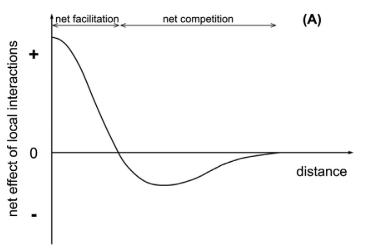
\includegraphics[scale=0.5]{sdf}
    \caption{Scale-dependent feedback}
    \label{fig:sdf}
\end{figure}

From the figure, there appears to be a maximum optimal distance wherein the negative effects of competition are minimized.
This model does not only work for mussel populations, but has been hypothesized for general populations \cite{Dong2019}.

\subsection{Community ecology}

One of the most common nonlinear system models in community ecology is the Lotka-Volterra model, also known as the predator-prey model \cite{Seibold2018}.
Without mathematical modeling, the scenario can be set up as follows:

\begin{itemize}
    \item Consider two trophic levels: prey and predator
    \item Suppose there is relatively fewer predators to prey
    \item Suppose once the prey supply decreases, its consumption also decreases
    leading to eventual population growth through reproduction
    \item While prey supply decreases, predator population growth also decreases
    \item Finally, as prey population increases predator population follows suit
\end{itemize}

It is evident from the third item that the \emph{sustainability} of the complex system relies on the reproductive rate of prey species and consumption rate of predator species.
Suppose the prey species produces at a much slower rate compared to the consumption rate of the predator species.
A simulation of the above interaction will intuitively lead to the extinction of the prey species, thus requiring the predator species to occupy a new niche.
In other words, changes in environmental or species parameters have led to system death.

Extending from a ``population'' interaction within colonies, another type of community interaction was discussed by \citeA{Dong2019}, wherein bacteria of different species were placed in one environment.
Patterns of self-organization were seen within colonies, which allowed for long-term equilibruim, while none were observed when the different bacteria were introduced.
The reviewers compared the observation to the economic ``tragedy of the commons''.
This may be the case when competing agents do not know how to interact with one another (a broad complex systems theory parameter).

By increasing the scale of the interactions: by increasing the number of trophic levels, by increasing the number of interacting species in specified trophic levels, by increasing the number of interactions being observed, or by combinations of the aforementioned methodologies, more complex interactions can be studied \cite{Seibold2018}.
The cited article appeals for more in-depth analysis from community ecology studies through multitrophic approaches.
One of the reasons said is worth quoting at length:

\begin{quote}
We live in an era where the accelerating loss of biodiversity due to overexploitation and loss of natural habitats, invasions, and climate change, as well as the effects of that loss on ecosystem processes and services, requires greater commitment to applied ecology to better provide guidance for dealing with these environmental issues.
\end{quote}

Anthropogenic interactions (human interventions) and their consequences, while considered as community ecological interactions, will be discussed in the last chapter of the reports.

\section{Self-organization in ecological systems}

The review by \citeA{Dong2019} encompassed different forms of self-organization in multiple levels of ecological organization.
Some of them are summarized as follows:

\paragraph{At the organismal level}
Self-organization at the organismal level is controlled by gene expression and the complex mechanisms behind epigenetics (\textit{ibid.}).
Such interactions form patters that appear as phenotypes may also be called \emph{adaptations} for the specific environment.

\paragraph{At the population level}
Self-organization of \textit{Mytilus edulis}, as discussed one of the previous sections, is driven by scale dependent feedback regulation (\textit{ibid.}).
This is done so that the population can be \emph{sustained}.

\paragraph{At the community level}
Complex interactions between different organisms and the abiotic environment occur including, but not limited to intra- and intertrophic interactions \cite{Seibold2018}, and competition \cite{Dong2019}.
The patterns form from sustainable \emph{niches} occupied by the interacting agents through coevolution.

\section{Bifurcations and catastrophes}

Bifurcations are a special term for significant changes in the way agents may asymptotically approach an optimal ``self-organized'' system.
These happen from significant changes in parameters dependent that control the properties of the agents.
In the figure below, a type of bifucation is shown.

\begin{figure}[h]
    \centering
    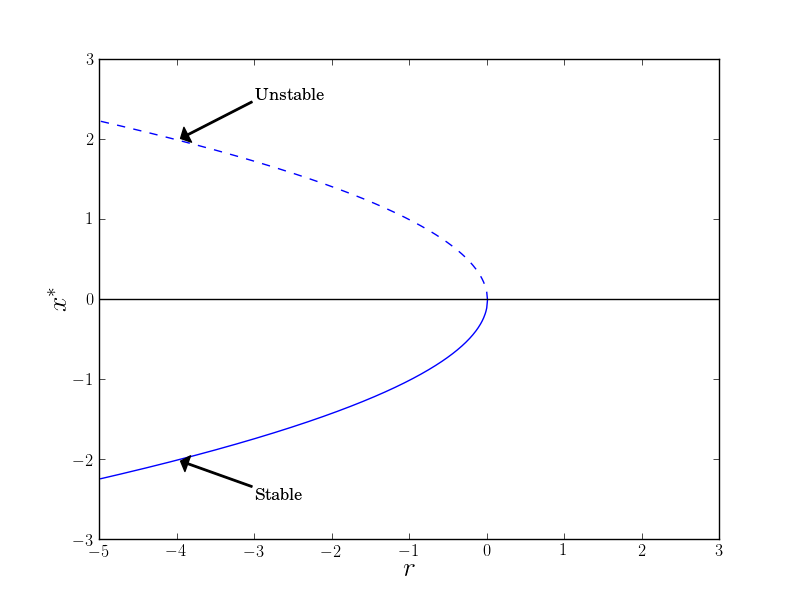
\includegraphics[scale=0.4]{sadd}
    \caption{A saddle node bifurcation}
    \label{fig:sadd}
\end{figure}

The saddle-node bifurcation is one of the simplest, yet most important bifurcation models.
In the bifurcation model, if the control parameter exceeds a threshold the loss of self-organization capabilities occurs and leads to system death (catastrophe) \cite{Devaney}.

In the case of intracellular systems, one such parameter may be related to the size of the cell and its use of resources.
This is an indirect conclusion from the above introduced study on metabolite-enzyme regulation study \cite{Chaves2019}.
Suppose there were mutations that allow for fast cell growth, requiring fast utilization of metabolites; however, other parameters such as the interaction of enzymes and substrates remain the same (\textit{ceteris paribus}).
Then there will come a point that the cell cannot sustain itself, and thus will result to its own destruction.
The study of how such parameters affect the system dynamics is in the realm of bifurcation theory, and will not be explored here (partly due to the lack of deeper knowledge of the researcher).

\section{Influences of self-organization on adaptation and evolution}
From the exposition of biological and ecological interactions between different agents in different levels of ecological organization.
Certain, some instantaneous, internal and environmental parameters influence the outcome of these agent interactions.
Systems can either organize by themselves forming patterns of self-organization or ultimately lead to catastrophes.

\paragraph{Synthesis}
What happens if gene mutation rates increased? It depends!
There are biological and ecological factors contributing to the complexity of the outcome.
What are the organisms? What are they subjected to?
How do they interact with their environment before the mutations?
Moreover... At what rate does the ``increased rate'' occur?
How will the gene regulatory networks be affected?
What will happen to the metabolic pathways of the organism given the unknown changes by the mutations?
Complexity in biological systems is ubiquitous, and it \emph{is} difficult to characterize with a lack of parameters of interest.
